\section{CP Violation in the \texorpdfstring{\BstoJpsiphi{}}{Bs0->Jpsiphi} Decay}
\label{sec:intro_Jpsiphi}

%%%%%%%%%%%%%%%%%%%%%%%%%%%%%%%%%%%%%%%%%%%%%%%%%%%%%%%%%%%%%%%
\subsection{The \texorpdfstring{\BsBsbar{}}{Bs0-Bs0bar} System}
\label{subsec:intro_Jpsiphi_Bs}
%%%%%%%%%%%%%%%%%%%%%%%%%%%%%%%%%%%%%%%%%%%%%%%%%%%%%%%%%%%%%%%

The $\Bs$ meson is a QCD bound state of an anti-b quark and an s quark. Its antiparticle is the $\Bsbar$ meson (b and anti-s). The $\Bs$
and $\Bsbar$ are charge-neutral particles, which makes it possible to convert one into the other. Figure~\ref{fig:mixing} shows the
lowest-order diagrams for this transition.
\begin{figure}[hbt]
  \centering
  \begin{subfigure}{0.5\textwidth}
    \centering
    {\sffamily \documentclass[11pt]{standalone}
\usepackage{color}
\usepackage[cmyk]{xcolor}
\usepackage{feynmp}
\usepackage{graphicx}
\usepackage{amsmath}
\usepackage{libertine}
\DeclareGraphicsRule{*}{mps}{*}{}

\newcommand{\Bs}{\text{B}_\text{s}^\text{0}}
\newcommand{\Bsbar}{\kern 0.06em \overline{\kern -0.06em \Bs \kern -0.32em} \kern 0.32em}

\begin{document}
\sffamily
\begin{fmffile}{./box1}
  \fmfframe(19,3)(17,3){
    \begin{fmfgraph*}(115,75)
      \fmfbottom{i1,d1,o1}%dummy vertex
      \fmftop{i2,d2,o2}
      \fmf{fermion,label=s,l.side=left}{i1,v1}
      \fmf{fermion,label={t,,c,,u},l.side=left}{v1,v2}
      \fmf{fermion,label=b,l.side=left}{v2,o1}
      \fmf{fermion,label=b,l.side=left}{v3,i2}
      \fmf{fermion,label={t,,c,,u},l.side=left}{v4,v3}
      \fmf{fermion,label=s,l.side=left}{o2,v4}
      \fmffreeze
      \fmf{boson,label=W,l.side=left}{v1,v3}
      \fmf{boson,label=W,l.side=right}{v2,v4}
      \fmf{plain,left=0.2}{o1,o2}
      \fmf{plain,left=0.2,label=$\Bsbar$}{o2,o1}
      \fmf{plain,left=0.2}{i2,i1}
      \fmf{plain,left=0.2,label=$\Bs$}{i1,i2}
    \end{fmfgraph*}
  }
\end{fmffile}
\end{document}
}
    \label{fig:mixing_1}
  \end{subfigure}%
  \begin{subfigure}{0.5\textwidth}
    \centering
    {\sffamily \documentclass[11pt]{standalone}
\usepackage{color}
\usepackage[cmyk]{xcolor}
\usepackage{feynmp}
\usepackage{graphicx}
\usepackage{amsmath}
\usepackage{libertine}
\DeclareGraphicsRule{*}{mps}{*}{}

\newcommand{\Bs}{\text{B}_\text{s}^\text{0}}
\newcommand{\Bsbar}{\kern 0.06em \overline{\kern -0.06em \Bs \kern -0.32em} \kern 0.32em}

\begin{document}
\sffamily
\begin{fmffile}{./box2}
  \fmfframe(19,3)(17,3){
    \begin{fmfgraph*}(115,75)
      \fmfbottom{i1,d1,o1}%dummy vertex
      \fmftop{i2,d2,o2}
      \fmf{fermion,label=s,l.side=left}{i1,v1}
      \fmf{fermion,label=b,l.side=left}{v2,o1}
      \fmf{fermion,label=b,l.side=left}{v3,i2}
      \fmf{fermion,label=s,l.side=left}{o2,v4}
      \fmf{boson,label=W$^-$,l.side=left}{v1,v2}
      \fmf{boson,label=W$^+$,l.side=left}{v4,v3}
      \fmffreeze
      \fmf{fermion,label={t,,c,,u},l.side=left}{v4,v2}
      \fmf{fermion,label={t,,c,,u},l.side=left}{v1,v3}
      \fmf{plain,left=0.2}{o1,o2}
      \fmf{plain,left=0.2,label=$\Bsbar$}{o2,o1}
      \fmf{plain,left=0.2}{i2,i1}
      \fmf{plain,left=0.2,label=$\Bs$}{i1,i2}
    \end{fmfgraph*}
  }
\end{fmffile}
\end{document}
}
    \label{fig:mixing_2}
  \end{subfigure}
  \caption{Lowest-order diagrams for \BsBsbar{} mixing~\cite{LHCb-PAPER-2013-002}.}
  \label{fig:mixing}
\end{figure}

Their mixing makes the $\Bs$ and $\Bsbar$ a coupled system of particles. The system comprises two eigenstates with different masses and
mean lifetimes (see Section~\ref{sec:pheno_mix}). A particle that is created as $\Bs$ can be observed as either a $\Bs$ or a $\Bsbar$ at a
later point in time. As a result, the distribution of the time at which the \BsBsbar{} system decays is not a simple exponential, as it is
for a single particle. Because the expression for the probability to observe the system as a $\Bs$ or a $\Bsbar$ contains sinusoidal
terms in time, mixing is often referred to as ``\BsBsbar{} oscillations''.

The \emph{decay time} is defined as the time difference between the production and the decay of the \BsBsbar{} system in its rest frame. In
Section~\ref{sec:pheno_mix} the exact shape of the decay-time dependence will be discussed. The applied formalism is common to the $\Dmes$,
$\Bd$ and $\Bs$ mesons and, to some extend, also the $\kaon$ meson, which all mix with their respective antiparticles.

The parameters that are used to describe the \BsBsbar{} system are the mean decay width $\Gs$, the difference between the decay widths of
the eigenstates $\DGs$, and the difference between the masses of the eigenstates $\Dms$. By definition, the mean lifetime of the system is
given by $\taus$\textequiv$\frac{\text{1}}{\Gs}$. The mass difference will turn out to be the frequency of the oscillations of the
\BsBsbar{} probability in time.

In the Standard Model, CP violation enters the mixing process through the CKM-matrix elements at W-boson vertices. The amplitudes in
Figure~\ref{fig:mixing} depend on the mass of the internal up-type quark, which makes the \BsBsbar{} mixing process dominated by diagrams
with virtual top quarks. As a result, CP violation is small, since it requires multiple contributions with different weak phases. In terms
of Equation~\ref{eq:interference}, this corresponds to a small value of $R$, which suppresses the CP asymmetry.

The additional contributions that give rise to small \emph{CP violation in mixing} are transitions via real intermediate states into which
both $\Bs$ and $\Bsbar$ can decay, which will be discussed in more detail in Section~\ref{sec:pheno_mix}. The asymmetry between the
$\Bs\to\Bsbar$ and $\Bsbar\to\Bs$ rates is measured to be approximately one per cent~\cite{Amhis:2012bh}. This is compatible with no CP
violation given the current experimental uncertainties.

Depending on the final state, there may also be different amplitudes contributing to the decay of the $\Bs$ meson. Also then
interference can lead to different decay rates, in this case for the $\Bstof$ and $\Bsbartofbar$ processes. This form is termed \emph{CP
violation in decay}.

The first significant observation of CP violation in the $\Bs$ system was recently obtained by LHCb~\cite{LHCb-PAPER-2013-018}. This was a
measurement of CP violation in decay for $\Bsbar\to\Kp\pimes[-]$ and $\Bs\to\Km\pimes[+]$, where an asymmetry in the decay rates of about
30\% was found.

\newcommand{\ffig}{\fp}
\newcommand{\phimixfig}{\phi_\text{mix}}
\newcommand{\phifig}{\phi_\text{dec}}
\newcommand{\phibarfig}{\kern 0.15em \overline{\kern -0.15em \phi_\text{dec} \kern -0.60em} \kern 0.60em}
\begin{figure}[tb]
  \centering
  \resizebox{0.32\textwidth}{!}{\input{graphics/intro/decay.pdftex_t}}
  \caption{Interference between the $\Bstof[\fp]$ and $\Bs\to\Bsbartof[\fp]$ processes. The phases $\phimixfig$, $\phifig$, and
           $\phibarfig$ are the relevant weak phases contributing to the two decay paths from the mixing, $\Bs$ decay and $\Bsbar$ decay,
           respectively. This is assuming no CP violation in mixing or CP violation in decay.}
  \label{fig:interference}
\end{figure}

An interesting situation occurs if both $\Bs$ and $\Bsbar$ can decay into the same final state $\fp$. In that case the processes
$\Bstof[\fp]$ and $\Bs\to\Bsbartof[\fp]$ interfere, which is depicted schematically in Figure~\ref{fig:interference}. Even without CP
violation in mixing or CP violation in decay, the interference of these two decay paths may cause a difference between the rates of
$\Bs(\to\Bsbar)\to\fp$ and $\Bsbar(\to\Bs)\to\overline{\fp}$. This difference is called \emph{CP violation in the interference of decays
with and decays without mixing}.

Interference between the decays with and without mixing does not lead to a CP asymmetry in total decay rate, but to an asymmetry that
depends on decay time. A sinusoidal term is introduced in the differential decay rate in time with an amplitude that depends on the amount
of CP violation. This oscillation originates from the time dependence of the transition amplitudes in \BsBsbar{} mixing and consequently has
a frequency equal to the mass difference $\Dms$. In an experiment it is important to resolve the resulting oscillation in the decay-time
distribution, which enables the measurement of its amplitude and hence the amount of CP violation.

A special case of this form of CP violation is the one where $\fp$ is a CP eigenstate. In this case $\fp$ and $\overline{\fp}$ are
identical and CP violation results in a difference between the decay rates of $\Bs(\to\Bsbar)\to\fp$ and $\Bsbar(\to\Bs)\to\fp$.

An example of such a decay is the so-called ``golden mode'' \BdtoJpsiKS. The combination of CKM-matrix elements in $\Bd$--$\Bdbar$ mixing
and the \BdtoJpsiKS{} decay makes the amplitude of the oscillations in decay time depend on the CKM angle $\beta$. The measurement of
$\beta$ with this decay mode by the BaBar and Belle experiments~\cite{Aubert:2001nu,*Abe:2001xe} was the first observation of CP violation
in $\Bd$ decays. The result of combining all currently available measurements of the angle $\beta$~\cite{Amhis:2012bh} is consistent with
the value obtained from the global Standard Model fits~\cite{Charles:2004jd,Bona:2005vz}.


%%%%%%%%%%%%%%%%%%%%%%%%%%%%%%%%%%%%%%%%%%%%%%%%%%%%%%%%%%%%%%%%
\subsection{\texorpdfstring{\BstoJpsiphi{}}{Bs0->Jpsiphi} Decay}
\label{subsec:intro_Jpsiphi_decay}
%%%%%%%%%%%%%%%%%%%%%%%%%%%%%%%%%%%%%%%%%%%%%%%%%%%%%%%%%%%%%%%%

The \BstoJpsiphi{} decay%
\footnote{Charge-conjugate particles, CP-conjugate decays and neutral-meson mixing are implied, unless stated otherwise.}
of the $\Bs$ system is equivalent to the \BdtoJpsiKS{} decay of the $\Bd$ system. Its decay-time distribution depends on the angle $\bs$
instead of $\beta$, as will be shown below.

However, a complication arises in comparison to \BdtoJpsiKS{} from the fact that both the $\Jpsi$ and the $\phimesalt$ are spin-one mesons,
whereas the $\KS$ is a spin-zero meson. This leads to three possible orbital angular momentum configurations of the $\Jpsiphi$ system,
compared to one configuration for the $\Jpsi\,\KS$ system. As a result, the \BstoJpsiphi{} decay comprises three different CP eigenstates
instead of one. The contributions of these states must be statistically separated by an analysis of the $\Jpsi$ and $\phimesalt$ spin
polarizations for an optimal measurement~\cite{Dighe:1995pd,*Dighe:1998vk}, as will be explained in Section~\ref{sec:pheno_decay}.

\begin{figure}[hbt]
  \centering
  \begin{subfigure}{0.5\textwidth}
    \centering
    {\sffamily \documentclass[11pt]{standalone}
\usepackage{color}
\usepackage[cmyk]{xcolor}
\usepackage{feynmp}
\usepackage{graphicx}
\usepackage{amsmath}
\usepackage{libertine}
\DeclareGraphicsRule{*}{mps}{*}{}

\newcommand{\Bs}{\text{B}_\text{s}^\text{0}}
\newcommand{\Bsbar}{\kern 0.06em \overline{\kern -0.06em \Bs \kern -0.32em} \kern 0.32em}

\begin{document}
\sffamily
\begin{fmffile}{./tree}
  \fmfframe(17,-25)(31,-25){
    \begin{fmfgraph*}(115,170)
      \fmfstraight
      \fmfleft{i0,i1,i2,i3,i4,i5}
      \fmfright{o0,o1,o2,o3,o4,o5}
      \fmf{fermion,tension=3.5,label.side=left,label=b}{v2,i3}
      \fmf{fermion,label=c,label.side=left}{o4,v2}
      \fmf{fermion,label=c,label.side=left}{v3,o3}
      \fmf{fermion,label=s,label.side=left,tension=2}{o2,v3}
      \fmf{boson,tension=2.4,label=W$^+$,label.side=right,right=0.3}{v2,v3}
      \fmffreeze
      \fmf{phantom,tension=0.3}{v2,v1,v3}
      \fmf{fermion,tension=0.5,label=s,label.side=left}{v1,o1}
      \fmf{fermion,tension=0.5,label.side=left,label=s}{i2,v1}
      \fmf{plain,right=0.2}{i2,i3}
      \fmf{plain,left=0.2,label=$\Bs$}{i2,i3}
      \fmf{plain,right=0.2}{o1,o2}
      \fmf{plain,left=0.2}{o1,o2}
      \fmf{plain,right=0.2}{o3,o4}
      \fmf{plain,left=0.2}{o3,o4}
    \end{fmfgraph*}
  }
\end{fmffile}
\end{document}
}
    \caption{}
    \label{fig:decay_tree}
  \end{subfigure}%
  \begin{subfigure}{0.5\textwidth}
    \centering
    {\sffamily \documentclass[11pt]{standalone}
\usepackage{color}
\usepackage[cmyk]{xcolor}
\usepackage{feynmp}
\usepackage{graphicx}
\usepackage{amsmath}
\usepackage{libertine}
\DeclareGraphicsRule{*}{mps}{*}{}

\newcommand{\Bs}{\text{B}_\text{s}^\text{0}}
\newcommand{\Bsbar}{\kern 0.06em \overline{\kern -0.06em \Bs \kern -0.32em} \kern 0.32em}

\begin{document}
\sffamily
\begin{fmffile}{./penguin}
  \fmfframe(17,-25)(31,-25){
    \begin{fmfgraph*}(115,170)
      \fmfstraight
      \fmfleft{i0,i1,i2,i3,i4,i5}
      \fmfright{o0,o1,o2,o3,o4,o5}
      \fmf{fermion,tension=1.8,label.side=left,label=b}{v5,i3}
      \fmf{fermion,tension=1.5,right=0.2,label.side=left,label={\hspace*{18pt}u,,c,,t}}{v2,v5}
      \fmf{gluon,tension=2}{v4,v2}
      \fmf{dbl_dashes,tension=0}{v4,v2}
      \fmf{fermion,tension=0.3,right=0.2,label.side=left }{v3,v2}
      \fmf{boson,tension=0.6,left=0.3,label=W$^+$,label.side=left}{v3,v5}
      \fmf{fermion,label=c,tension=0.9,right=0.3,label.side=left}{o4,v4}
      \fmf{fermion,label=c,tension=0.9,right=0.3,label.side=left}{v4,o3}
      \fmf{fermion,label=s,label.side=left}{o2,v3}
      \fmffreeze
      \fmf{fermion,tension=0.7,label=s,label.side=left}{v1,o1}
      \fmf{fermion,tension=1,label.side=left,label=s}{i2,v1}
      %\fmf{phantom,tension=0.4}{v4,v1}
      \fmf{phantom,tension=0.4}{v3,v1,v5}
      \fmf{plain,right=0.2}{i2,i3}
      \fmf{plain,left=0.2,label=$\Bs$}{i2,i3}
      \fmf{plain,right=0.2}{o1,o2}
      \fmf{plain,left=0.2}{o1,o2}
      \fmf{plain,right=0.2}{o3,o4}
      \fmf{plain,left=0.2}{o3,o4}
    \end{fmfgraph*}
  }
\end{fmffile}
\end{document}
}
    \caption{}
    \label{fig:decay_penguin}
  \end{subfigure}
  \caption{\BstoJpsiphi{} decay: (a) tree-level diagram; (b) penguin diagram~\cite{LHCb-PAPER-2013-002}. The curled/dashed line in (b)
           represents a colour-neutral state, which can be a Z$^0$, a photon, or colour-singlet gluons.}
  \label{fig:decay}
\end{figure}
At quark level, the \BstoJpsiphi{} decay is a \emph{$\btoccs$ transition}. The b quark decays into an s quark and a c$\qbar[c]$ pair, where
the s quark forms a $\phimesalt$ meson with the spectator $\qbar[s]$ quark and the c$\qbar[c]$ pair forms a $\Jpsi$ meson.
Figure~\ref{fig:decay_tree} shows the dominant Standard Model contribution. This is a tree-level diagram, which is proportional to the
CKM-matrix elements $\Vcs$ and $\Vcb[*]$.

Since the CP-violation phenomenology is governed by \BsBsbar{} mixing and the $\btoccs$ transition, decays where the c$\qbar[c]$ and
s$\qbar[s]$ pairs form different mesons may be used in addition to \BstoJpsiphi. An important example is the \BstoJpsipipi{}
decay~\cite{Stone:2008ak}, from which he value of $\phis$ can be obtained with a precision that is comparable to the precision in the
\BstoJpsiphi{} channel.

The dominant contributions to the \BsBsbar{} mixing with internal top quarks (Figure~\ref{fig:mixing}) are proportional to
$(\Vts\Vtb[*])^2$. In combination with the tree-level decay, it gives a weak phase difference between decays with and decays without mixing
of
\begin{equation}
  \label{eq:betasCKM}
  \begin{split}
    &\arg\left[(\Vts\Vtb[*])^2\right] + \arg\left(\Vcs[*]\Vcb\right) - \arg\left(\Vcs\Vcb[*]\right) \\
    &\qquad\qquad= 2\,\arg\left(-\frac{\Vts\Vtb[*]}{\Vcs\Vcb[*]}\right) = 2\bs
    \ ,
  \end{split}
\end{equation}
where the first contribution comes from the $\Bs\to\Bsbar$ transition, the second contribution from the subsequent $\Bsbar$ decay, and the
third contribution from the $\Bs$ decay path without mixing.

Additional contributions to the mixing and decay processes can affect this estimate of the weak phase. The quantity that is observed in
this measurement is the phase $\phis$, which is equal to --2$\bs$ with the above assumptions.%
\footnote{There are various, often contradicting notations of the phase difference in use. In this work $\bs$ is the CKM-triangle angle
(Equation~\ref{eq:bsAnglesDef}) and $\phis$ the model-independent observable (see Section~\ref{sec:pheno_decay}). If only dominant
Standard Model contributions to both mixing and decay are considered, $\phis$ is equal to --2$\bs$.}

In the Standard Model, corrections come from the mixing diagrams with real states and from higher order contributions to the decay.  While
the former lead to small Standard Model CP violation in mixing, these amplitudes are not expected to contribute significantly to the value
of $\phis$ (see Section~\ref{sec:pheno_mix_obs}). An example of an additional contribution to the decay is the \emph{penguin diagram} in
Figure~\ref{fig:decay_penguin}. Although hard to estimate, small contributions from penguin diagrams to the decay are
expected~\cite{Faller:2008gt,*Bhattacharya:2012ph}.

Beyond the Standard Model, CP violation can arise from new contributions to the \BsBsbar{} mixing
process~\cite{Nir:1990hj,*Silverman:1998uj,*Ball:1999yi,*Dunietz:2000cr,Buras:2009if} as well as the $\Bs$
decay~\cite{Chiang:2009ev,*Datta:2009fk}. In general it is expected that potential corrections to the Standard Model are largest in
processes with virtual particles in loops at lowest order. Loop processes are smaller than tree-level processes, which makes Standard Model
contributions compete with potential new contributions at the same level. New particles must be heavy and cannot be created in decays of
Standard Model particles. In loop processes, however, they can enter as virtual particles and replace, for example, the internal top quarks
in the \BsBsbar{} mixing diagrams. For these reasons, the focus of the measurement will be on mixing-induced CP violation rather than CP
violation that arises from the \BstoJpsiphi{} decay, which is dominated by the tree-level amplitude in Figure~\ref{fig:decay_tree}.

If the effect of new contributions on the value of $\phis$ is large compared to the Standard Model value, the corresponding deviation can
be revealed by the measurement of a large non-zero value of $\phis$. In this case an exact estimate of the Standard Model value is not
required and subleading penguin contributions can be neglected. In addition, a large deviation could be detected by a low-statistics
measurement, which would not have the precision to distinguish between the cases of no CP violation, the Standard Model, and a small
deviation from the Standard Model.

Measurements of $\phis$ with the \BstoJpsiphi{} decay have been performed by the D0~\cite{Abazov:2011ry}, CDF~\cite{Aaltonen:2012ie},
\atlas~\cite{Aad:2012kba,*ATLAS:2013nla}, and LHCb~\cite{LHCb-PAPER-2013-002} experiments. LHCb also measured $\phis$ in the
\BstoJpsipipi{} decay channel~\cite{LHCb-PAPER-2014-019}. All measurements and their combination~\cite{Amhis:2012bh} are compatible with no
CP violation and also with the value of $\bs$ from the Standard Model fit. The LHCb measurement in the \BstoJpsiphi{} channel yielded
\begin{equation}
  \label{eq:phis1fb}
  \phis\text{\texteq+0.07\textpm0.09$\,$(stat.)\textpm0.01$\,$(syst.)~~rad\ ,}
\end{equation}
where the first uncertainty is statistical and the second systematic. This value is to be compared with the Standard Model estimate
--2$\bs$\texteq--0.0368$^\text{+0.0013}_\text{--0.0014}$\unitsp{}rad (see Equation~\ref{eq:CKMAnglesCKMf} and
reference~\cite{Charles:2004jd}).

A measurement of the decay-time distribution in \BstoJpsiphi{} is not only sensitive to the phase $\phis$, but also to the lifetime
parameters of the \BsBsbar{} system. The previously mentioned CP violation measurements yielded estimates of $\Gs$ and $\DGs$ as well.
These parameters were also estimated by CMS in a measurement that assumed no CP violation~\cite{CMS:2012pca}.

In the Standard Model the parameter $\Gs$ is expected to be equal to the $\Bd$ decay width, $\Gd$, up to relative corrections of the order
of \tenpow{--3}~\cite{Lenz:2006hd,*Lenz:2011ti}. $\Gd$ is measured to be 0.6583\textpm0.0030\unitsp\invps~\cite{Amhis:2012bh}. A prediction
of the decay-width difference $\DGs$ yields 0.087\textpm0.021\unitsp\invps~\cite{Lenz:2006hd,*Lenz:2011ti}. The measurements of $\Gs$ and
$\DGs$ and their combination~\cite{Amhis:2012bh} are compatible with these predictions. The estimates from the LHCb measurement are given
by
\begin{subequations}
  \label{eq:width1fb}
  \begin{align}
    \label{eq:avWidth1fb}
    \Gs&\text{\texteq0.663\textpm0.005$\,$(stat.)\textpm0.006$\,$(syst.)~~\invps} \\
    \label{eq:diffWidth1fb}
    \DGs&\text{\texteq0.100\textpm0.016$\,$(stat.)\textpm0.003$\,$(syst.)~~\invps\ .}
  \end{align}
\end{subequations}

\begin{figure}[tb]
  \centering
  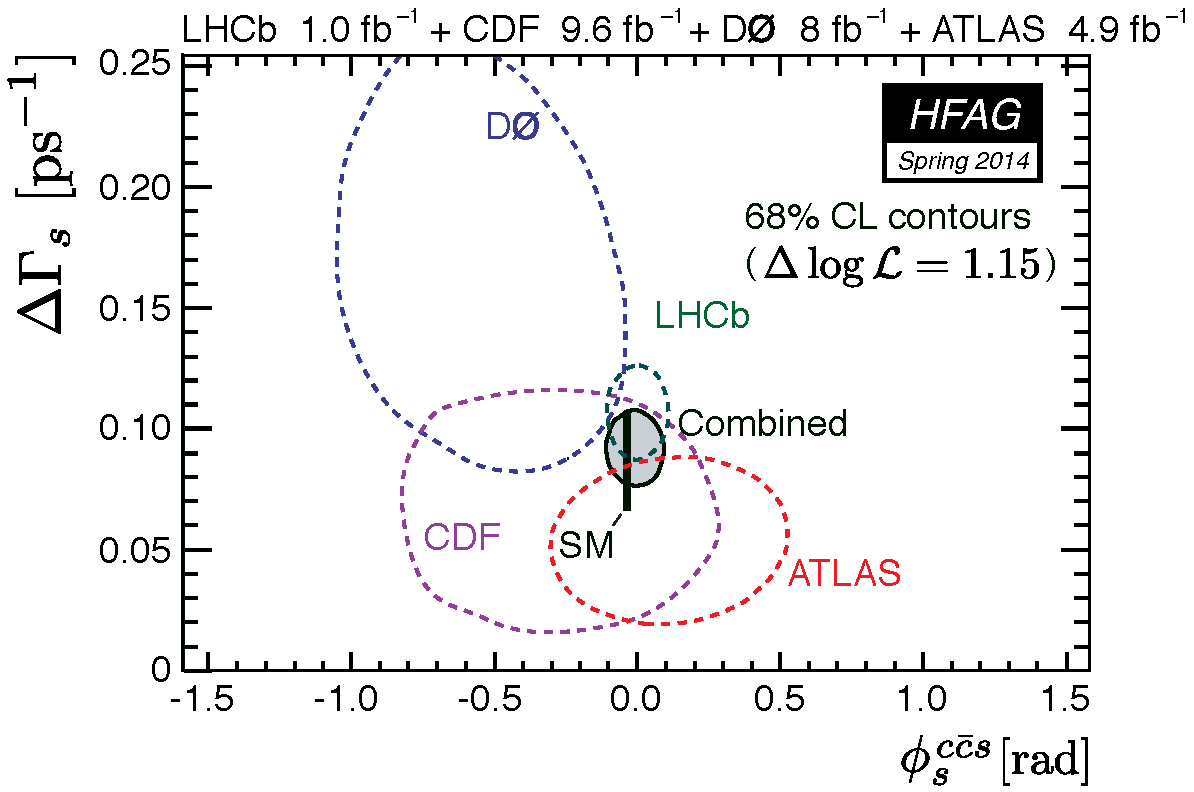
\includegraphics[width=0.8\textwidth]{graphics/intro/hfag_spr2014_DGsphis_comb-crop-cmyk}
  \caption{Combination of $\phis$ (here represented as $\phisccs$) and $\DGs$ measurements by HFAG~\cite{Amhis:2012bh}.
           The estimates at 68\% confidence level (CL) by the different experiments are shown by the dashed contours.
           Note that the LHCb contour is a combination of measurements in the \BstoJpsiphi{} and \BstoJpsipipi{} decays.
           The combined 68\% confidence region is shown by the shaded area and the Standard Model prediction by the vertical bar.}
  \label{fig:phisDGs}
\end{figure}
A graphical representation of the status of $\phis$ and $\DGs$ measurements in the spring of 2014 by the Heavy Flavour Averaging Group
(HFAG) is shown in Figure~\ref{fig:phisDGs}. The LHCb contribution is a combination of the \BstoJpsiphi{} and \BstoJpsipipi{} results with
data from 2011, which form roughly one third of the currently available dataset. The 68\% confidence-level (CL) contour of the combined
result is consistent with the region that represents the Standard Model prediction.

As it is clear from Figure~\ref{fig:phisDGs} that possible effects from non-Standard Model physics on $\phis$ and $\DGs$ cannot be large,
more precise measurements are needed to probe them. With the currently available LHCb data, combination of the $\phis$ estimates from the
two decay channels is expected to reach a precision of approximately 0.04~rad, which is roughly equal to the value of the Standard Model
prediction. An improvement of this precision by an order of magnitude is expected with future LHCb data.

For a measurement with this precision, effects have to be taken into account that have not been considered for previous measurements. A
precise estimate of Standard Model CP violation is required, which also includes higher order penguin contributions to the $\btoccs$
transition. A problem arises from the fact that these additional contributions affect the value of $\phis$ differently for the
\BstoJpsiphi{} and \BstoJpsipipi{} decays and for the different intermediate states that contribute to the
decays~\cite{Faller:2008gt,*Bhattacharya:2012ph}. Moreover, physics beyond the Standard Model may also affect all intermediate states
differently~\cite{Chiang:2009ev,*Datta:2009fk}. These effects need to be considered not only in theoretical predictions, but also in
measurements.

In the \BstoJpsiphi{} measurement that is presented in this thesis the dependence of CP violation on the intermediate state is taken into
account for the first time. The value of $\phis$ is estimated separately for each of the CP eigenstates in the decay, which is possible
if the contributions of the states are statistically separated. The decay model for this measurement is presented in
Chapter~\ref{chap:pheno}.


%%%%%%%%%%%%%%%%%%%%%%%%%%%%%%%%%%%%%%%%%%%%%%%%%%%%%%%%%%%%%%%%%%%
\subsection{The \texorpdfstring{$\mumuKK$}{mu+mu-K+K-} Final State}
\label{subsec:intro_Jpsiphi_final}
%%%%%%%%%%%%%%%%%%%%%%%%%%%%%%%%%%%%%%%%%%%%%%%%%%%%%%%%%%%%%%%%%%%

The $\Jpsiphi$ system is unstable and only its decay products can be detected. There are many possibilities for both the $\Jpsi$ and
$\phimesalt$ mesons to decay~\cite{PDG}. The only final state that will be considered here is $\mumu\,\KK$, where the muon pair
originates from the $\Jpsi$ decay and the kaon pair from the $\phimesalt$ decay. All four particles can be detected efficiently and with
low background by the LHCb detector, as will be described in Section~\ref{sec:intro_LHCb}. This makes \BstoJpsimumuphiKK{} the optimal
channel to measure CP violation in $\Bs$ decays with a $\btoccs$ transition.

Since the $\mumuKK$ final state can also be reached through resonances other than the $\Jpsi$ and the $\phimesalt$, interference with other
processes needs to be considered. To optimize for the detection of the $\Jpsi$ and $\phimesalt$ resonances, a region in kinematic phase
space is selected where this intermediate state dominates.

The measured invariant mass of the muon pair is required to be between 3.03 and 3.15~\GeV{} (see also Section~\ref{sec:exp_selBkg}).
%\footnote{The unit of energy used in particle physics is the \emph{electronvolt} (eV), which is approximately equal to
%1.6\tenpowmult{--19}~J. Derived units for momentum and mass are \eVc{} and \eV, respectively, where $c$ is the speed of light.}
This restriction is assumed to select only those \BstomumuKK{} decays with muons coming from a $\Jpsi$, which has a mass of approximately
3.10~\GeV{}~\cite{PDG}.

Also the invariant-mass range of the $\KK$ pair is restricted, but there the situation is more complicated. An analysis of the resonant
components in the $\KK$ system~\cite{LHCb-PAPER-2012-040} has shown that there is a mass region where the $\phimes$ dominates, but other
contributions cannot be neglected.

\begin{figure}[tb]
  \centering
  %\begin{tikzpicture}[line width=0.08em]
  %  \node [anchor=south] {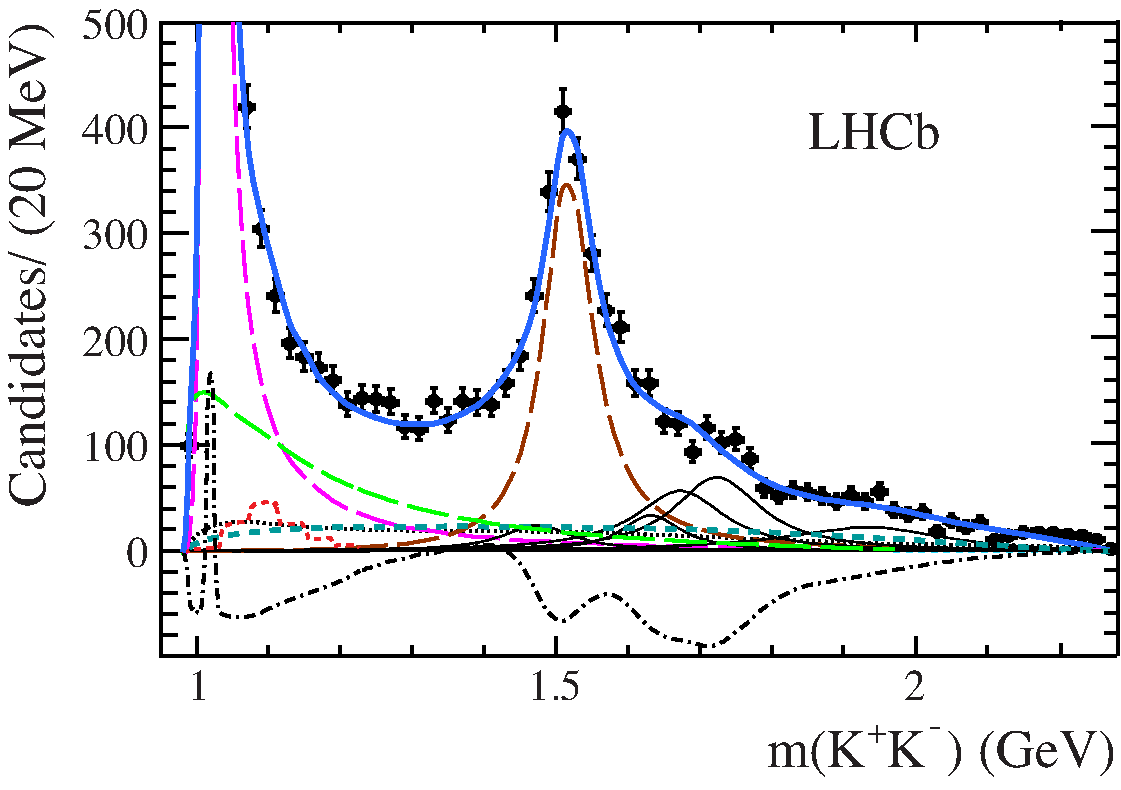
\includegraphics[width=0.7\textwidth]{graphics/intro/KKComponents}};
  %  \draw[red] (-0.2047\textwidth,0.04\textwidth) -- (-0.2047\textwidth,0.52\textwidth);
  %\end{tikzpicture}

  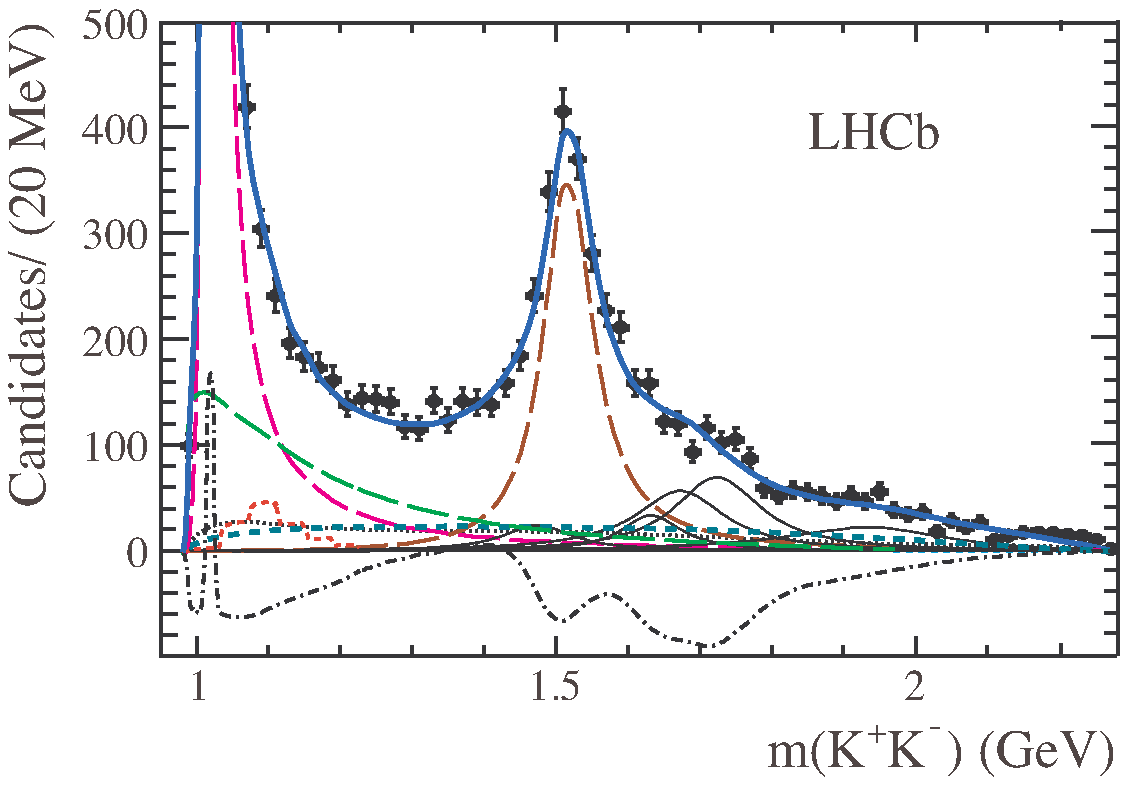
\includegraphics[width=0.85\textwidth]{graphics/intro/KKComponents-cmyk}
  \caption{$\KK$-mass spectrum in \BstoJpsiKK{} decays~\cite{LHCb-PAPER-2012-040}. The black points represent a histogram of decay
           candidates.
           %, where the size of the error bar shows the fluctuation expected from a Poisson distribution of the number of entries
           %in each mass bin.
           A model of the mass distribution is shown as the blue curve. The largest contributions to the distribution
           come from the $\phimes$, $\ftwop$, and $\fzero$ resonances, which are shown as the magenta,
           brown, and green long-dashed lines, respectively. Notice that a large part of the $\phimes$ peak is not visible,
           because of the truncated vertical scale.
           Other resonances are shown as the thin, black curves and a non-resonant
           contribution as the dashed, cyan curve. Contributions from interferences between the resonances are represented
           by the dotted-dashed, black line. The small dotted, black and dashed, red contributions are backgrounds of four
           particles that do not originate from a \BstoJpsiKK{} decay.}
           %The region to the left of the vertical, red line is dominated by the $\phimes$.}
  \label{fig:KKComponents}
\end{figure}

The $\KK$-mass spectrum in \BstoJpsiKK{} decays is shown in Figure~\ref{fig:KKComponents}. The contribution of the $\phimes$ is represented
by the dashed, magenta curve. Notice that part this peak is not visible, because of the truncated vertical scale.

For the \BstoJpsiphi{} CP-violation measurement, only $\KK$ pairs with a mass between 0.99 and 1.05~\GeV{} are selected. In this region the
$\phimes$ clearly dominates, but there are also contributions from the $\fzero$ and from $\KK$ pairs that do not originate from the decay
of a resonance.

The $\KK$ system is in a state of zero orbital angular momentum for both of the additional non-$\phimesalt$ contributions and hence they
are referred to as the \emph{$\KK$ S-wave}. Because the $\Jpsiphi$ and $\KK$ S-wave processes are observed simultaneously in a measurement,
the analysed decay is referred to as \BstoJpsiKK.

In addition to separating the three components of the \BstoJpsiphi{} process, these components are also separated from the two S-wave
contributions. The latter could be accomplished on a statistical basis with an analysis of the $\KK$-mass distribution. However, this
distribution does not discriminate between the CP eigenstates of the \BstoJpsiphi{} decay, so a different approach is chosen.

Because the $\phimes$ is a spin-one particle, the orbital angular momentum of the $\KK$ system has a P-wave configuration for the
$\Jpsiphi$ intermediate state. This makes the spatial distributions of the final-state particles different from the S-wave distributions,
which enables a statistical separation of the two components. An analysis of the spatial distributions also separates P-wave
spin-polarization states and hence the three CP eigenstates of the $\Jpsiphi$ system.

The directions of the final-state particles are specified with respect to the momentum directions of the $\mumu$ and $\KK$ systems in the
centre-of-mass system of the $\Bs$ meson. This is done with three \emph{decay angles}, which can be computed given the four-momenta of the
final-state particles. These angles are included in the model of the decay, in addition to the decay time. The formalism for the angular
dependence of the decay is described in detail in Section~\ref{sec:pheno_angles} and Appendix~\ref{chap:angularDecay}.
